\documentclass[12pt, oneside]{article}
\usepackage{geometry}                		% See geometry.pdf to learn the layout options. There are lots.
\geometry{letterpaper} 
\usepackage{amsmath}
\usepackage{amsthm}
\usepackage{amssymb}
\usepackage{graphicx}
\usepackage{color}
\usepackage{float}
\usepackage{subfig}
\usepackage[flushleft]{threeparttable}
\usepackage{gensymb}
\usepackage{multirow}
\usepackage[dvipsnames]{xcolor}
\newcommand{\BibTeX}{\textsc{Bib}\TeX}
%opening
\title{VDS_HDF5}
\author{}

\begin{document}


\section{What this Tool does}
This tool is used to make a virtual data set. A virtual data set is a grouping of links to multiple data files. 
The benefit of this is you can assemble these data sets into 1 data file much faster than making that file would take, 
additionally that file will be significantly smaller.

\begin{figure}[H]
\centering
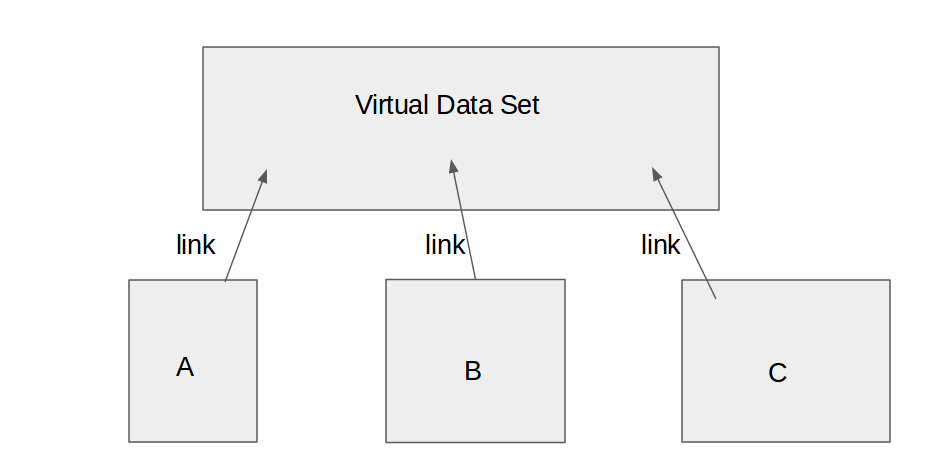
\includegraphics[width=0.5\textwidth]{FIGS/VDS_assembly.png}

\caption{{\footnotesize Example of VDS Creation}}
\label{fig: } 
\end{figure}


\section{Compiling the Code}
This code makes use of a newer version of the HDF5 library than is currently implemented. So in order to compile this code you will need to remake all used code
using a compatible version, ie HDF5\_1.10. To assist in this the make clean function of the make file will also clean out the modules directory.

To recompile first make clean the directory, then you will need to change the library location used in the makecomm.inc file to where the HDF5\_1.10 library is located.
After this use the make command to compile the code.

\section{Using the Code}
In order to use this code define the max variables which define the size of the VDS, this should correspond to the dimensions of the completed file.
Additionally choose the format that corresponds with the format of the files to be combined. Lastly define the flowdata numbers.








\end{document}